\chapter{Inequality}% by Zim-mim Siddiqee Sowdha}
\begin{linkb}
   \begin{itemize}
        \item \href{https://www.youtube.com/watch?v=H7UwnAGZY0A}{Inequality (Sowdha)} 
        \item \href{https://drive.google.com/file/d/1Vm117lBF5yuZrRGMjmMS-HccPmknl5uK/view?usp=sharing}{Apply AM-GM ...}
        \item \href{https://drive.google.com/file/d/12GWPOw5_9c4-KD5PNCdJSS0i3lAORI5s/view}{P set}
   \end{itemize}
\end{linkb}
%\section{Some Theorems and Lemmas}
\section{Triangle inequality}
 In euclidean geometry,for any triangle with side $a$, $b$,$c$,
 \[a+b >c\] 
and \[a-b<c\] and so on.

In vector space the triangle inequality also holds. Which means, when $a$ and $b $ are vectors then,
\[|a+b| \le |a|+|b|\]
 and \[|a-b|\ge ||a|-|b||\]
 
  This is true for any real number $a$ and $b$ where $|a|$ is the absolute value of $a$. Because, 
  \[ (a+b)^2 = |a|^2+ |b|^2 + 2ab \le |a|^2 + 2|a||b| + |b|^2 = (|a|+|b|)^2  \]
  \[\implies |a+b|^2 \le  (|a|+|b|)^2 \]
  \[\implies |a+b| \le  (|a|+|b|) \]
  The other one can be proved similarly. 
 
 
    \section{Some classic definitions of means}
    \begin{definition}[Root Mean Square]
    Root mean square of $a_1, \cdots ,a_n$ positive real numbers defined as,
    \[\sqrt {\frac{a_1^2+ \cdots +a_n^2}{n}}\]
    This is also known as quadratic mean.
    \end{definition}
\begin{definition}[Arithmetic Mean ]
Arithmetic mean of $a_1, \cdots ,a_n$ positive real numbers defined as, 
\[ \frac{a_1+...+a_n}{n}\]
\end{definition}
\begin{definition}[Geometric Mean]
Geometric mean of $a_1, \cdots  ,a_n$ positive real numbers defined as, 
   \[ (a_1 \cdots a_n)^{\frac{1}{n}} \]
\end{definition}
\begin{definition}[Harmonic Mean]
Geometric mean of $a_1, \cdots  ,a_n$ positive real numbers defined as,
\[\frac{n}{\frac{1}{a_1}+\cdots+ \frac{1}{a_n}}\]
\end{definition}
  
 \begin{theorem}[RMS-AM-GM-HM inequality]
 For positive reals $a_1, \cdots  ,a_n$ we have
        \[\sqrt {\frac{a_1^2+ \cdots +a_n^2}{n}} \ge \frac{ a_1+...+a_n}{n} \ge (a_1 \cdots a_n)^{\frac{1}{n}} \ge \frac{n}{\frac{1}{a_1}+\cdots+ \frac{1}{a_n}} \]
 \end{theorem}
%\begin{theorem}[Triangle inequality]
%for 2 vectors $a$ and $b$, 
%\[|a+b|\le|a|+|b|\]
%\end{theorem}
 %   This inequality is true for all real number $a, b$%
 
\section {A fun proof of RMS-AM-GM-HM}
We present a geometric proof of RMS-AM-GM-HM inequality for $n=2$.Let $a,b $ be two real numbers then. Consider the following diagram,
\begin{figure}[ht]
\centering
    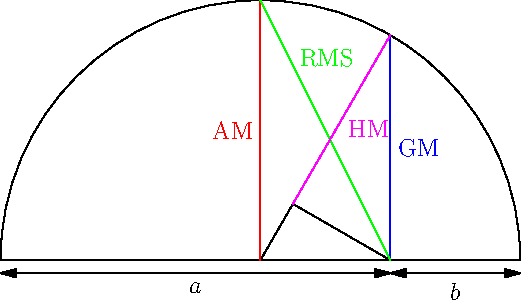
\includegraphics{am-gm.pdf}
    \label{label of the figure}         
\end{figure}
It is left as an exercise to figure out why this lines refer to the corresponding meaning. 
Now it is easy to see that why this inequality is true for $n=2$. 

\section{Example Problems}

\begin{example}
$\frac{m}{n}<\sqrt{2}$ if and only if  $\sqrt{2} < \frac{m+2n}{m+n}$

\end{example}
\begin{soln}
    For the if part, \[ \frac{m}{n}<\sqrt{2} \]
    \[ \implies  \frac{m}{n} +1 < \sqrt{2} +1\]
    \[ \implies \frac{1}{\frac{m}{n} +1 }> \frac{1}{\sqrt{2}+1} \]
    \[ \implies 1 + \frac{1}{\frac{m}{n} +1 }> 1 +\frac{1}{\sqrt{2}+1} \]
    \[ \therefore \frac{m+2n}{m+n} > \sqrt {2} \]
    For the only if part, just go backwards. Which completes the proof.
\end{soln}


\begin{example}
$x,y,z $ are positive real numbers. Prove that,
\[\frac{xy}{z}+\frac{yz}{x}+\frac{zx}{y}\ge x+y+z\]
\end{example}
 \begin{soln}
 Here by AM-GM, we get ,
 \[\frac{xy}{z}+\frac{yz}{x}\ge 2 \sqrt {\frac{xy.yz}{z.x}}= 2y\]
 Similarly,
 \[\frac{yz}{x}+\frac{zx}{y}\ge 2z\]
     \[ \frac{zx}{y}+\frac{xy}{z} \ge 2x\]
     Then add these 3 inequalities will give the desired inequality. And we are done!
 \end{soln}
\begin{example}
Let $x,y $ be positive integers. Prove that, 
\[\frac{1}{x} + \frac{1}{y} \ge \frac{4}{x+y}\]
\end{example}

\begin{soln}
Notice that by AM-GM we get, 
\[(x+y) \ge 2 \sqrt{xy}\]
\[\implies (x+y)^2 \ge 4xy\]
Now multiply both side with $\frac{1}{xy(x+y)} $
\[\frac{x+y}{xy} \ge \frac{4}{x+y}\]
\[\implies \frac{1}{x} + \frac{1}{y} \ge \frac{4}{x+y}\]
Which is exactly what we wanted!

\end{soln}
However there is an another solution of this problem,
\begin{soln}
Take $a=\frac{x+y}{x}, b = \frac {x+y}{y}$. 
Now, by AM-GM we get, 
\[ a+b\ge 2\sqrt{ab}\]
\[\implies \frac{x+y}{x} + \frac{x+y}{y}\ge 2\sqrt{\frac{(x+y)^2}{xy}}=\frac{2(x+y)}{\sqrt{xy}} \]
Since, $x+y\ge 2\sqrt {xy}\implies \frac {x+y}{\sqrt{xy}}\ge 2  $. So, 
\[\frac{x+y}{x} + \frac{x+y}{y}\ge \frac{2(x+y)}{\sqrt{xy}}\ge 4\]
Divide both side by $(x+y)$. And we are done!

\end{soln}



\begin{example}
For $a\ge b> 0$. Prove that,
\[ \frac{1}{8}\frac{(a-b)^2}{a} \le \frac{a+b}{2} -\sqrt{ab} \le\frac{1}{8}\frac{(a-b)^2}{b}\]
\end{example}
 
 \begin{soln}
 We can modify this a bit, then it will look like 
 \[\frac{1}{8}\frac{(a-b)^2}{a} \le \frac{a+b-2\sqrt{ab}}{2} \le\frac{1}{8}\frac{(a-b)^2}{b}\]
 Or, \[\frac{1}{4}\frac{(a-b)^2}{a} \le (\sqrt{a}-\sqrt {b})^2 \le\frac{1}{4}\frac{(a-b)^2}{b}\]
We will first show that $\frac{1}{4}\frac{(a-b)^2}{a} \le  (\sqrt{a}-\sqrt {b})^2 $ and then we show that $  (\sqrt{a}-\sqrt {b})^2 \le \frac{1}{4}\frac{(a-b)^2}{b}$.
For the first part, notice that,
\[\sqrt{a} + \sqrt {b} \le 2\sqrt {a}\]
\[\implies (\sqrt{a} + \sqrt {b})^2 \le 4a\]
\[\implies \frac{(\sqrt{a}+\sqrt{b})^2(\sqrt {a}- \sqrt {b})^2}{(\sqrt {a}- \sqrt {b})^2}\le 4a\]
\[\implies \frac{(a-b)^2}{(\sqrt{a}- \sqrt {b})^2}\le 4a \]
    \[\implies \frac{(a-b)^2}{4a}\le (\sqrt{a}- \sqrt {b})^2\]
    So, \[\frac{1}{4}\frac{(a-b)^2}{a} \le  (\sqrt{a}-\sqrt {b})^2\]
    The second part is quite similar, 
    here, 
    $2\sqrt{b}\le \sqrt{a}+ \sqrt{b}$. Which gives 
    \[4b\le(\sqrt{a}+ \sqrt{b})^2 \]
\[\implies 4b\le \frac{(\sqrt{a}+\sqrt{b})^2(\sqrt {a}- \sqrt {b})^2}{(\sqrt {a}- \sqrt {b})^2} \implies 4b\le \frac{(a-b)^2}{(\sqrt{a}- \sqrt {b})^2} \implies (\sqrt{a}- \sqrt {b})^2\le \frac{(a-b)^2}{4b}
    \] 
And we are done!
    
    
 \end{soln}
 
 
 
 
 
 
 
\section{Practise Problems}
\begin{problem}
    For real numbers $a,b,c$ prove that

\[| a | + | b | + | c | − | a + b | − | b + c | − | c + a | + | a + b + c | \ge 0 \]
\begin{hint}
\addhint{}
\addhint{}
\end{hint}
\end{problem}

\begin{problem}[IMO SL-1996]
     Let $a,b,c$ be positive real numbers such that $abc=1$. Prove that,
     \[\frac{ab}{a^5 +b^5 +ab}+  \frac{bc}{b^5+c^5 +bc} + \frac{ca}{c^5 +a^5 +ca} \le 1\]
     \begin{hint}
     \addhint{}
     \addhint{}
     \end{hint}
\end{problem}


\begin{problem}
     Let $a,b,c$ be positive numbers. Prove that,
     \[\frac{2ab}{a+b}+\frac{2bc}{b+c} +\frac {2ca}{c+a}\le a+b+c \]
     \begin{hint}
     \addhint{}
     \addhint{}
     \end{hint}
\end{problem}


\begin{problem}
     If $a, b, c > 0$, prove that
     \[ \frac{1}{a}+ \frac{1}{b}+ \frac{1}{c}\ge 2 \left(\frac{1}{a+b} + \frac{1}{b+c}+ \frac{1}{c+a} \right) \ge \frac{9}{a+b+c} \]
     \begin{hint}
\addhint{}
\end{hint}
\end{problem}


\begin{problem}
     Let, $x_{1}, x_2, ..., x_n > 0 $ such that $\frac{1}{1+x_{1}}+ \cdots +\frac{1}{1+ x_{n}}=1$. Prove that, 
     \[ x_{1}x_{2}...x_{n} \ge (n − 1)^n \]
     \begin{hint}
     \addhint{}
     \addhint{}
     \end{hint}
\end{problem}

\begin{problem}[IMO SL, 1998]
Let $a_{1},a_{2},\ldots ,a_{n}$ be positive real numbers such that $a_{1}+a_{2}+\cdots +a_{n}<1$. Prove that

\[ \frac{a_{1} a_{2} \cdots a_{n} \left[ 1 - (a_{1} + a_{2} + \cdots + a_{n}) \right] }{(a_{1} + a_{2} + \cdots + a_{n})( 1 - a_{1})(1 - a_{2}) \cdots (1 - a_{n})} \leq \frac{1}{ n^{n+1}}. \]

    \begin{hint}
        \addhint{}
        \addhint{}
    \end{hint}

     
\end{problem}


\begin{problem}[APMO,1991]
Let $a_1$, $a_2$, $\cdots$, $a_n$, $b_1$, $b_2$, $\cdots$, $b_n$ be positive real numbers such that $a_1 + a_2 + \cdots + a_n = b_1 + b_2 + \cdots + b_n$. Show that
\[ \frac{a_1^2}{a_1 + b_1} + \frac{a_2^2}{a_2 + b_2} + \cdots + \frac{a_n^2}{a_n + b_n} \geq \frac{a_1 + a_2 + \cdots + a_n}{2} \]
    \begin{hint}
    \addhint{}
    \addhint{}
    \end{hint}
\end{problem}


